\documentclass{report}

\usepackage{fullpage}
\usepackage[skip=4pt]{caption} % ``skip'' sets the spacing between the figure and the caption.
\usepackage{pgfplots}   % Needed for plotting
\usepackage{amsmath}    % Allows for piecewise functions using the ``cases'' construct
\usepackage{graphics,subcaption, cleveref} % ``subcaption'' and ``cleveref'' are needed for subfigure
\usepackage{grffile}   % Allows period in the graphics file name

\usepackage[obeyspaces,spaces]{url} % Used for typesetting with the ``path'' command
\usepackage[hidelinks]{hyperref}   % Make the cross references clickable hyperlinks
\usepackage[bottom]{footmisc} % Prevents the table going below the footnote


% Set up page formatting
\usepackage{fancyhdr} % Used for every page footer and title.
\pagestyle{fancy}
\fancyhf{} % Clears both the header and footer
\renewcommand{\headrulewidth}{0pt} % Eliminates line at the top of the page.
\fancyfoot[LO]{CMPS242 \textendash{} Homework \#1} % Left
\fancyfoot[CO]{\thepage} % Center
\fancyfoot[RO]{Stolman \& Hammoudeh} %Right

\renewcommand{\thesubfigure}{(\alph{subfigure})}
\captionsetup[sub]{labelformat=simple}

\renewcommand\thesection{\arabic{section}} % Prevent chapter number in section number.

\newcommand{\eref}[1]{(\ref{#1})}
\newcommand{\wstar}{\vec{w}^{\star}}
\newcommand{\norm}[1]{\left\lVert#1\right\rVert}
\newcommand{\includeLambdaPlot}[3]{  
\begin{subfigure}[t]{#2}
  \centering
  \includegraphics[width=1.0\textwidth]{img/test_train_compare_d=9_lambda=#1.pdf}
  \caption{$\lambda=#1$}\label{#3}
\end{subfigure}}

% Change interline spacing.
\renewcommand{\baselinestretch}{1.1}

\title{\textbf{CMPS242 Homework \#1 \textendash{} Polynomial Learning}}
\author{Andrew Stolman \\~\\ \& \\~\\Zayd Hammoudeh}

\graphicspath{{img/}}
\begin{document}
  \maketitle
  
 
  \section{Homework Objective}
  
  The goal of this homework is to implement an algorithm that can learn the scalar weights of a {$9^{\text{th}}$-order} polynomial function with a single independent variable.  We also study the effect of a regularizing constant,~$\lambda$, on over-fitting.
  
  \section{Experiment Setup}
  
  We implemented our solver in both Python (with NumPy) and Matlab; the latter implementation provides better results so only Matlab results are discussed.  
  
  \subsection{Definition of $\wstar$}
  
  Certain $n$-degree polynomials can be modeled by the simple univariate vector space,~$P$.  For the independent variable,~$x$, the vector space's basis,
  
  \begin{equation}
    basis(P)=\langle 1,x,...,x^{n}\rangle,
  \end{equation}
  
  \noindent
  is dimension~$n+1$.  Given a member of the vector space,~${\vec{x} \in P}$, the resulting polynomial function is:
  
  \begin{equation}
    y=\vec{w}^{\text{T}}\vec{x},
  \end{equation}\label{eq:polynomial}
  
  \noindent
  where $\vec{w}$ is a vector of scalar weights with dimension~$n+1$.
  
  Given a set of examples, $(x_{i},t_{i})$,~$i=1...m$, define~$X$ as an $(n+1)$~by~$m$ matrix whose $i^{\text{th}}$ column is the vector in space~$P$ that corresponds to example value~$x_{i}$.  Define  $\vec{t}$ as the vector whose value at index~$i$ is~$t_{i}$.  The linear system in Eq.~\eref{eq:polynomial} then becomes:
  
  \begin{equation}
    \vec{y}=\vec{w}^{\text{T}}X
  \end{equation}\label{eq:tensorFunction}
  
  \noindent
  %this following paragraph isn't quite right, the equation which follows it minimizes the regularized error function, not RMS, and we actually haven't so far stated what the regularized error function is
  As proven in the homework description, the weight vector,~$\wstar$, that minimizes the root mean square~(RMS) error of Eq.~\eref{eq:tensorFunction} is
  
  \begin{equation}
    \wstar=(XX^{\text{T}} + \lambda I)^{-1}Xt,
  \end{equation}\label{eq:wstarDef}
  
  \noindent
  where~$\lambda$ is a regularizing constant and~$I$ is the $(n+1)$~identity matrix.
  
  \subsection{Improving the Calculation of $\wstar$ through Linear Solving}
  
  In the homework dataset, values in~$X$ range approximately from~${2*10^{-7}}$ to~${8*10^{8}}$.  Hence, calculating~$\wstar$ is greatly affected by floating point errors.  As such, when trying to find the inverse matrix ${(XX^{\text{T}} + \lambda I)^{-1}}$, Matlab warns that the matrix is ``\texttt{near singular or badly scaled}''  and further warns the ``results may be inaccurate.''  Python reports a similar warning.  As such, rather than finding~$\wstar$ through straight matrix multiplication, our implementation instead finds~$\wstar$ by solving the linear system:
    
  \begin{equation}
    (XX^{\text{T}} + \lambda I)\wstar=Xt
  \end{equation}
  
  \noindent
  This approach generally has lower error for this homework (by up to two orders of magnitude when $n=19$).  From a theoretical perspective, our revised technique is equivalent.
      
  \section{Effect of the Regularizer~$\lambda$}
  
  The regularizer,~$\lambda$, in Eq.~\eref{eq:wstarDef} prevents overfitting by preferring models with smaller values of~$\norm{w}$.  In our experiments, we tested different values of~$\lambda$ from the set, ${\{0\} \cup \{2^{i} | i=-10...10\}}$.  Figure~\ref{fig:tenFoldCv} shows the training, validation, and test errors with these values of~$\lambda$ for $10$-fold cross-validation.  For training and validation, the line represents the mean RMS-error while the bars are the variance.  The $x$~and $y$~axes are logarithmic for clearer visualization.\footnote{For this dataset, there are multiple values of~$\lambda$ where the validation variance exceeded its associated mean.  In such cases, the standard error bar plotting technique would have indicated the occurrence negative error, which is both impossible and non-graphable when using a logarithmic scale.  As such, we chose to visualize this phenomenon by clamping all negative variance bars at~$10^{-2}$.  We found this was clearer than leaving those negative error bars out entirely.}
  
  \begin{figure*}
    \centering
    \begin{subfigure}[t]{0.45\textwidth}
      \centering
      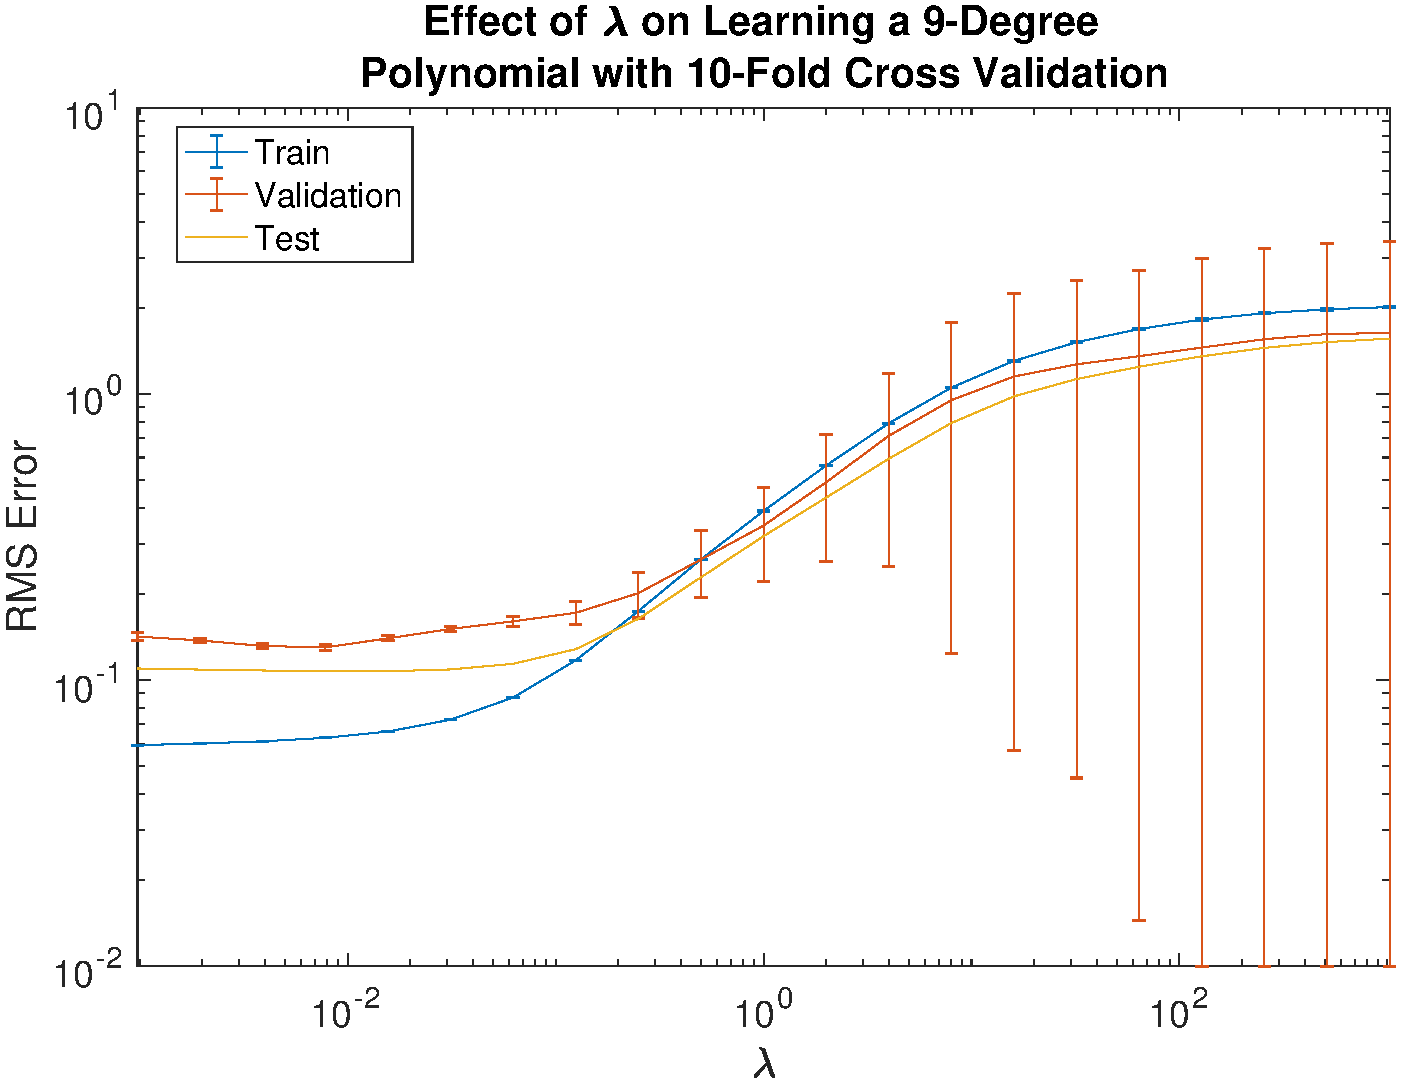
\includegraphics[width=1.0\textwidth]{img/lambda_sweep_k=10_degree=9.pdf}
      \caption{$k=10$}\label{fig:tenFoldCv}
    \end{subfigure}%
    ~ 
    \begin{subfigure}[t]{0.45\textwidth}
      \centering
      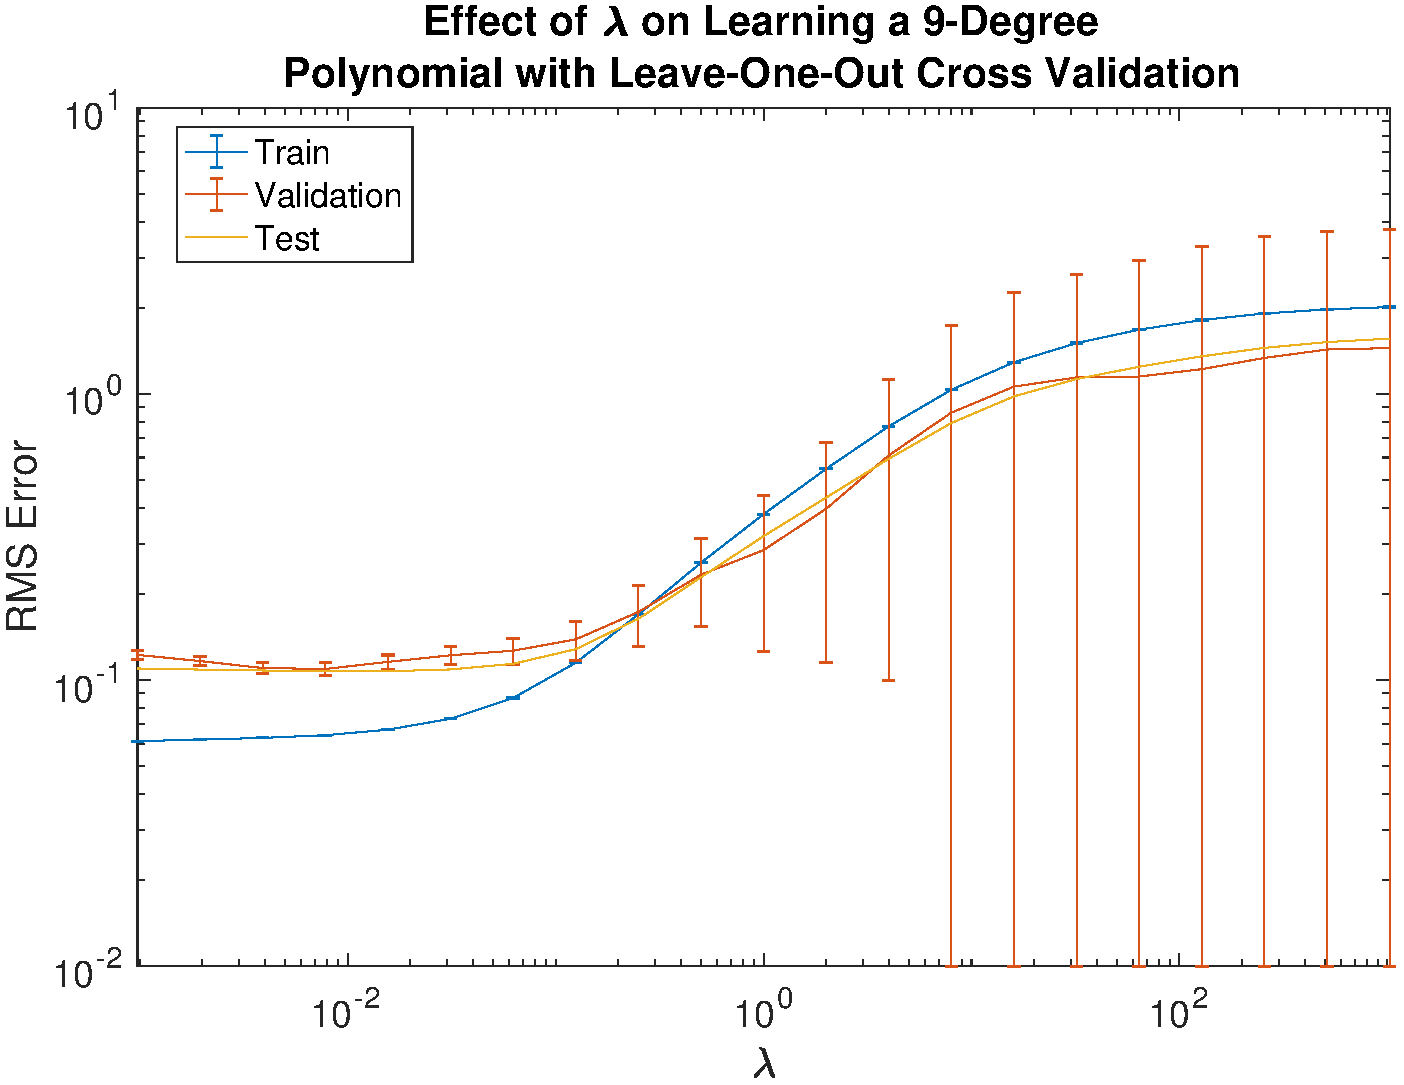
\includegraphics[width=1.0\textwidth]{img/lambda_sweep_leave_one_out_degree=9.pdf}
      \caption{Leave-One-Out}\label{fig:leaveOneOutCv}
    \end{subfigure}
    \caption{Effect of $\lambda$ and Cross Validation Fold Count when Learning a $9^{\text{th}}$-Order Polynomial}\label{fig:effectLambda}
  \end{figure*}


  \subsection{Selecting the Optimal Regularize}\label{sec:selectOptimalRegularizer}
  
  The selected value of the regularizer,~$\lambda$, should minimize or nearly minimize the validation error.  Table~\ref{tab:lambda10FoldError} shows the relationship between training, validation, and test errors for different values of~$\lambda$ when performing $10$-fold cross validation; optimal values are \textbf{bolded}.   Only values of~$\lambda \leq 2^{-6}$ are included in this table as Figure~\ref{fig:tenFoldCv} showed this range had the best overall performance.
  
  \begin{table}[b]
    \centering
    \caption{Learning Errors for Different Values of~$\lambda$ for 10-Fold Cross-Validation}\label{tab:lambda10FoldError}
    \label{my-label}
    \begin{tabular}{c||c|c|c|c|c|c|c}
      \hline
      $\lambda$  & 0     & $2^{-10}$ & $2^{-9}$ & $\mathbf{2^{-8}}$ & $2^{-7}$ & $2^{-6}$ & $2^{-5}$ \\ \hline\hline
      Training   & \textbf{0.057} & 0.059     & 0.060    & 0.061    & 0.063    & 0.066    & 0.073    \\ \hline
      Validation & 0.198 & 0.143     & 0.138    & \textbf{0.132}    & 0.133    & 0.141    & 0.148    \\ \hline
      Test       & 0.117 & 0.110     & 0.109    & 0.108    & \textbf{0.107}    & \textbf{0.107}    & 0.109    \\ \hline
    \end{tabular}
  \end{table}
  
  When a regularizer is not used (i.e.,~$\lambda=0$), the learning algorithm performs sub-optimally as indicated by the higher test error~(0.117). The regularizer,~$\lambda=2^{-8}$, had the minimum validation error for $10$-fold CV; its test error is also close to, but not exactly, the minimum.
  
  \subsection{Cross-Validation Fold Count}\label{sec:cvFoldCount}
  
  Figures~\ref{fig:tenFoldCv} and~\ref{fig:leaveOneOutCv} shows a comparison of the~$10$-fold and leave-one-out (LOO) cross-validation (CV) results respectively.  As expected, LOO~CV has higher variance in particular at large values of~$\lambda$; this can be seen visually since the error bars are longer.  The reason for the increase is because when the validation set is smaller in size, the validation error of outliers becomes more prominent.  Despite that, LOO~CV produces better results because first the mean validation error decreased and more importantly is closer to the actual test error.
  
  Table~\ref{tab:lambdaLooError} shows a comparison of the training, validation, and test errors when performing LOO~CV; optimal values are again shown in \textbf{bold}.  Note that unlike $10$-fold CV, LOO~CV resulted in the selection of the optimal value of~$\lambda$.
  
   \begin{table}[tb]
    \centering
    \caption{Learning Errors for Different Values of~$\lambda$ for Leave-One-Out Cross-Validation}\label{tab:lambdaLooError}
    \begin{tabular}{c||c|c|c|c|c|c|c}
      \hline
      $\lambda$  & 0     & $2^{-10}$ & $2^{-9}$ & $2^{-8}$ & $\mathbf{2^{-7}}$ & $2^{-6}$ & $2^{-5}$ \\ \hline\hline
      Training   & \textbf{0.059} & 0.061      & 0.062     & 0.063     & 0.064          & 0.067    & 0.073   \\ \hline
      Validation & 0.165          & 0.123      & 0.117     & 0.110     & \textbf{0.109} & 0.116    & 0.122   \\ \hline
      Test       & 0.117          & 0.110      & 0.109     & 0.108     & \textbf{0.107} & \textbf{0.107}    & 0.109   \\ \hline
    \end{tabular}
  \end{table}

  
  \section{Visualizing the Learner Outputs}
  
  As mentioned previously, our system learns a polynomial function.  Figure~\ref{fig:learnerTargetAndPredicted} compares the target (i.e.,~actual) and learned/predicted values for both the training and test sets.  Note that subfigures~\subref{fig:learnedZeroLambda},~\subref{fig:learnedTwoPowN8Lambda}, and~\subref{fig:learnedTwoPowN7Lambda} are for~$\lambda$ values of~$0$,~$2^{-8}$, and~$2^{-7}$ respectively.  These result visually align with the RMS errors reported in sections~\ref{sec:selectOptimalRegularizer} and~\ref{sec:cvFoldCount}.  Recall that~${\lambda=0}$ had a suboptimal test error; the cause of this can be seen in the slight hook in the graph when~$x$ is close to zero as well as the overshoot at the local maximum around~${x=6}$.  Similarly, the results for~$\lambda$ equal to~$2^{-8}$ and~$2^{-7}$ are very similar with no perceptible differences; this is expected as their test errors differed by less than~$0.6\%$.
  
  \begin{figure*}[h]
    \centering
    \includeLambdaPlot{0}{0.3\textwidth}{fig:learnedZeroLambda}
    ~ 
    \includeLambdaPlot{2^{-8}}{0.3\textwidth}{fig:learnedTwoPowN8Lambda}
    ~
    \includeLambdaPlot{2^{-7}}{0.3\textwidth}{fig:learnedTwoPowN7Lambda}
    \caption{Comparison of the Target and Predicted Values for Different Values of $\lambda$}\label{fig:learnerTargetAndPredicted}
  \end{figure*}

\section{Regularizing Without Bias}
We repeated the above process but modified the error function so that the constant term of the polynomial model would not be penalized. This is achieved by calculating the following error function:
\[ Err(\mathbf{w}) = ||\mathbf{X}^{T} \mathbf{w}-\mathbf{t}||^{2} + \lambda \langle \mathbf{0}_{1}, \mathbf{w} \rangle^{2}\]
where $\mathbf{0}_{1}$ refers to the vector with a zero in this first index and 1 everywhere else. Taking the derivative and setting it zero and solving gives us
\[ \wstar=(XX^{\text{T}} + \lambda I^{*})^{-1}Xt \textrm{,}\]
where $I^{*}$ is the identity matrix with the first row set to all zeros. 

The results are summarized in figure \ref{fig:withoutbias}.

\begin{figure*}[h]
\centering
\begin{subfigure}[h]{ 0.5\linewidth}
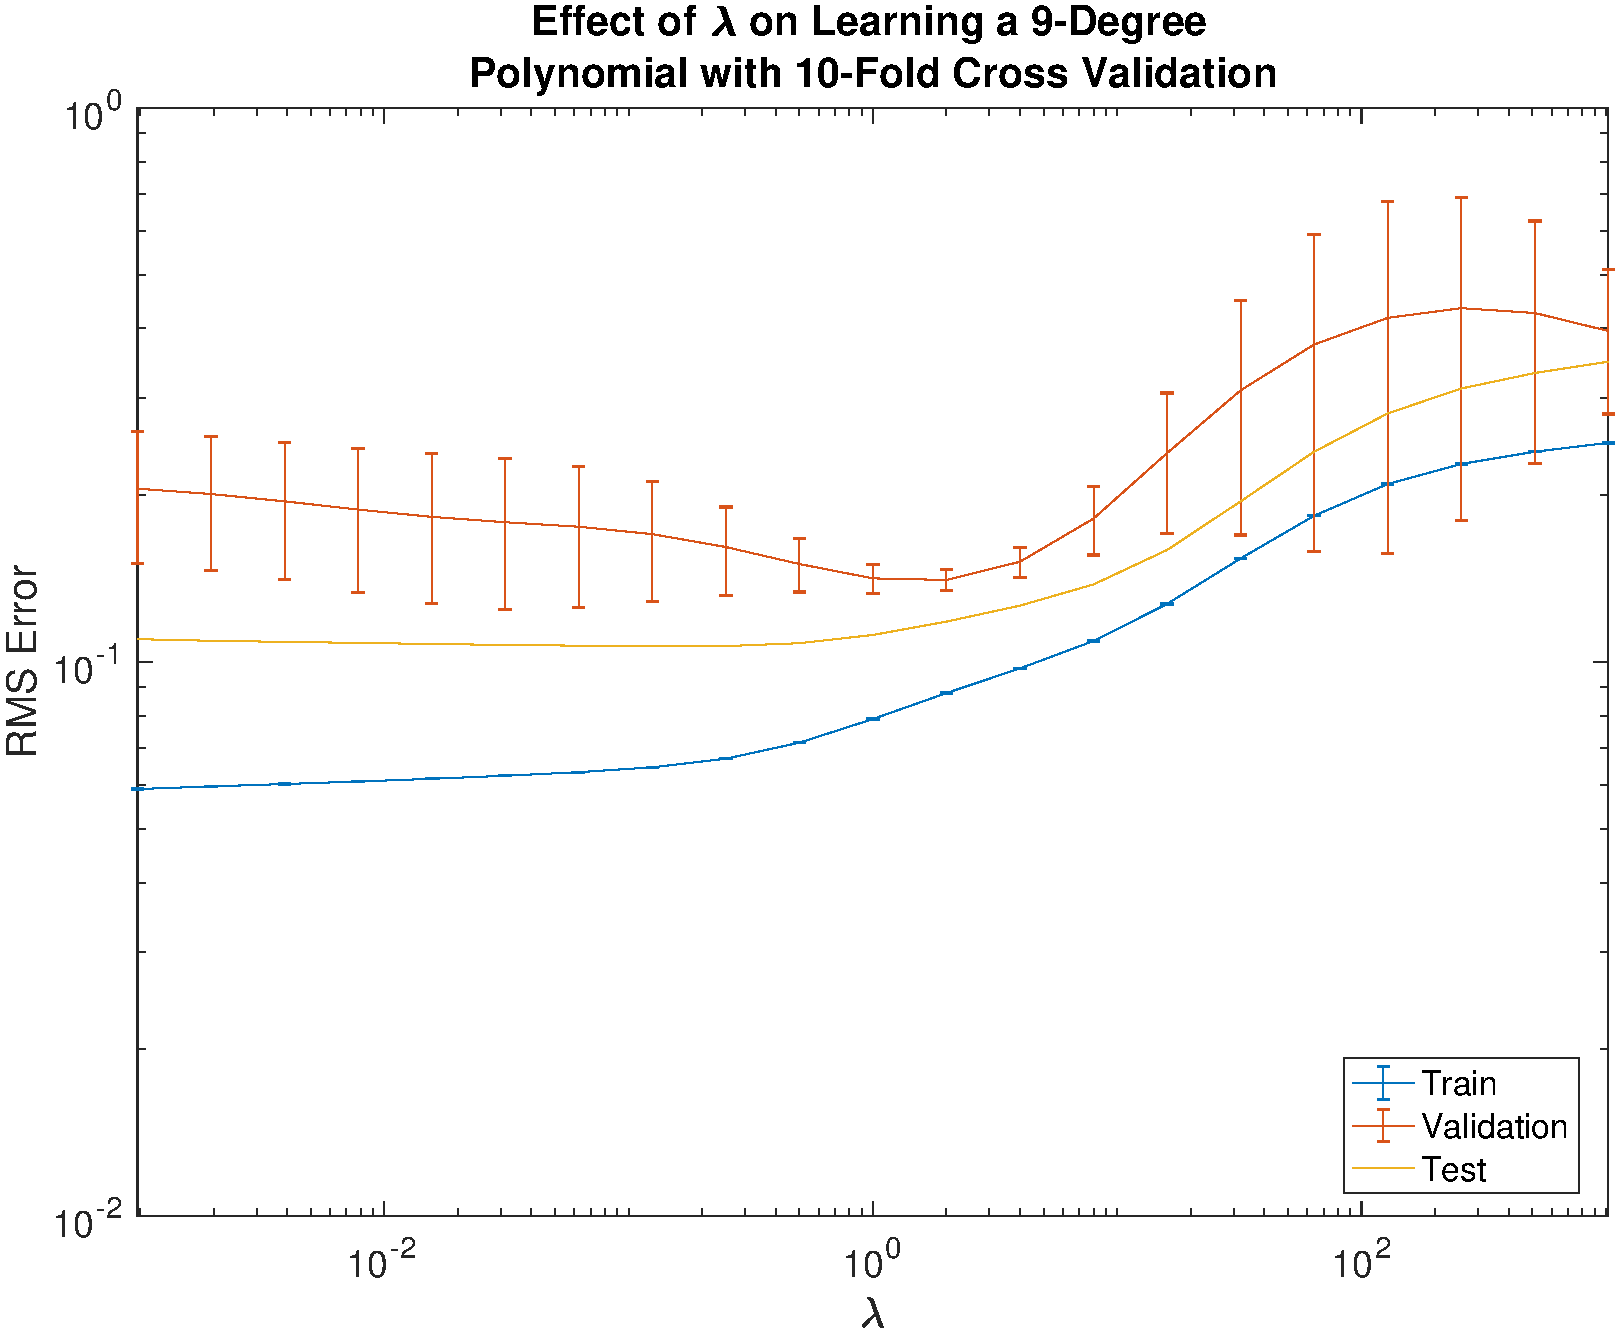
\includegraphics [width=\linewidth ]{lambda_sweep_without_bias}
\end{subfigure}
\begin{subfigure}[h]{ 0.5\linewidth}
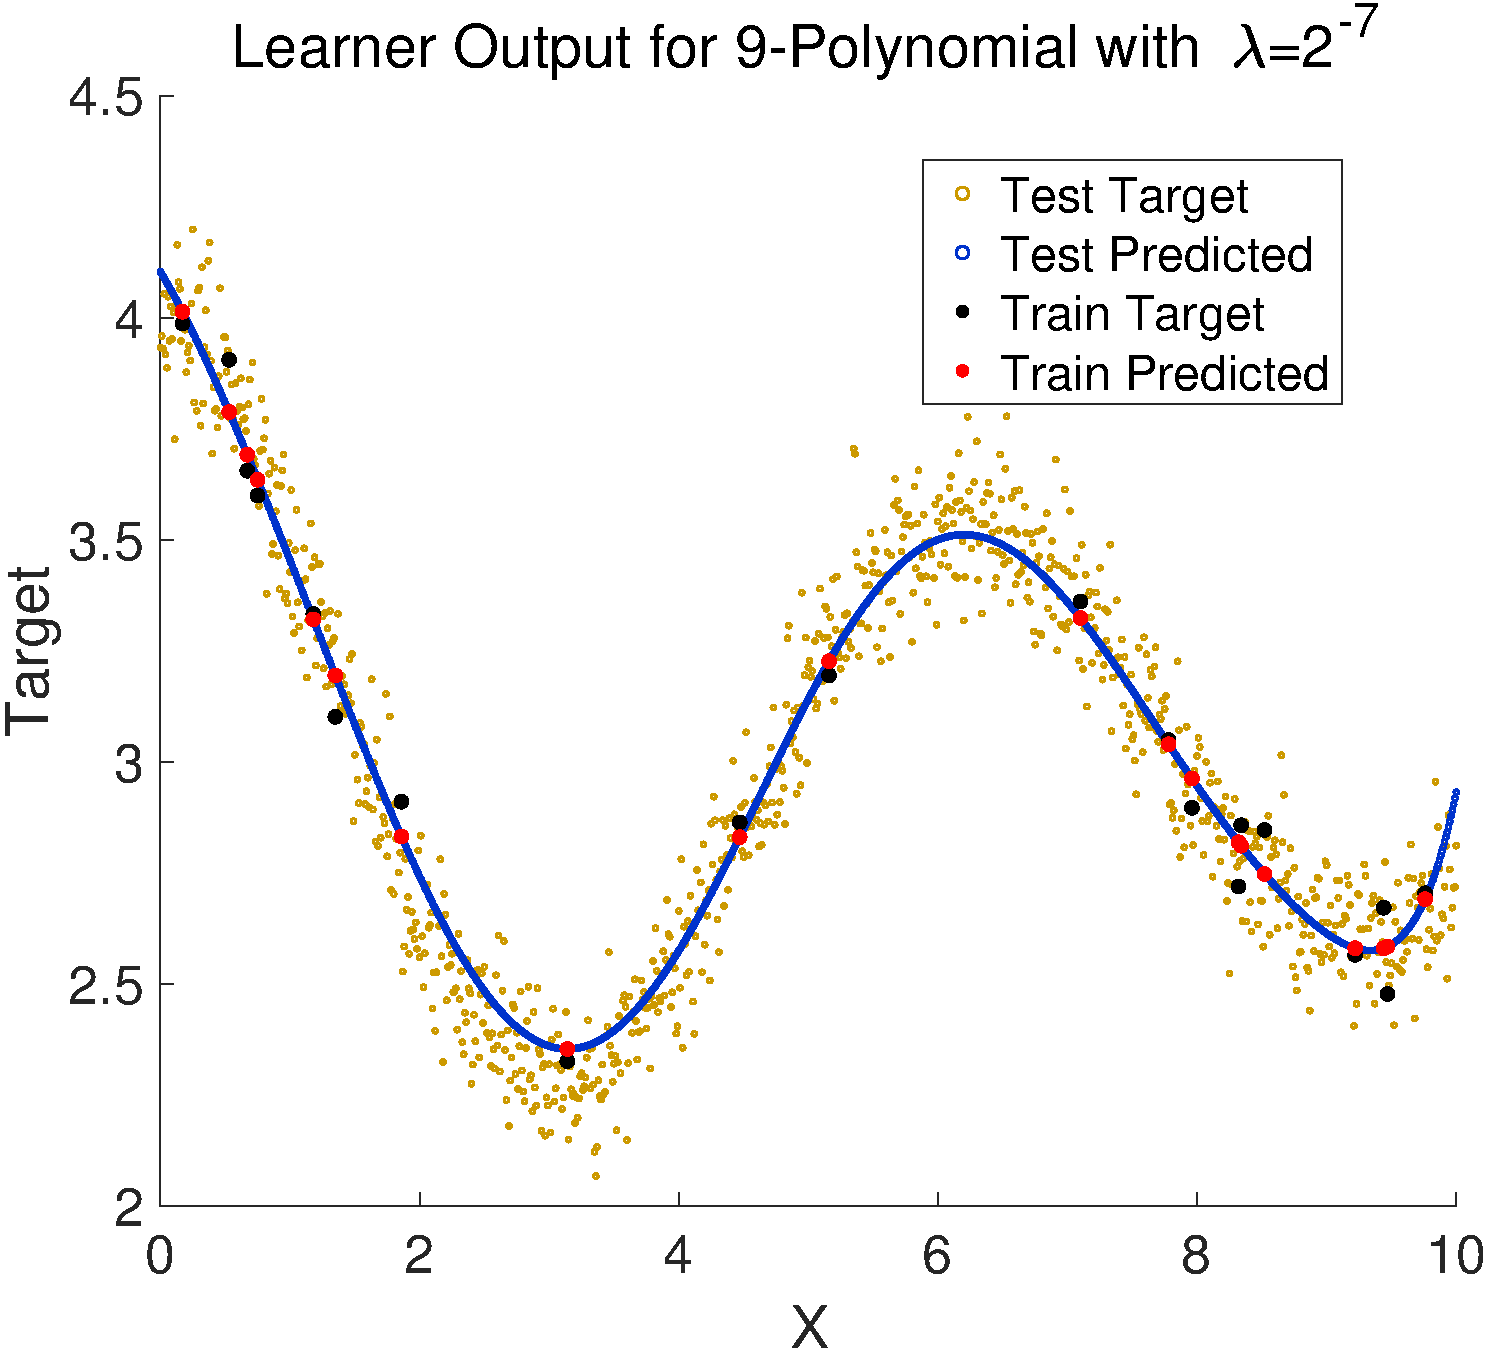
\includegraphics [width=\linewidth ]{without_bias_comparison}
\end{subfigure}
\label{fig:withoutbias}
\caption{Results for estimation without the bias term}
\end{figure*}

\end{document}